\documentclass{beamer}

\usepackage{amssymb, amsmath}
%\usepackage[all]{xy}

\usepackage{alltt}
\usepackage{pslatex}
\usepackage{epigraph}
\usepackage{verbatim}

%\usepackage{graphicx}
\usepackage{latexsym}
\usepackage{array}
\usepackage{comment}
\usepackage{makeidx}
\usepackage{listings}
\usepackage{indentfirst}
\usepackage{verbatim}
\usepackage{color}
\usepackage{url}
\usepackage{xspace}
%\usepackage{fontspec}
%\usepackage{xunicode}
%\usepackage{xltxtra}
%\usepackage{xecyr}
\usepackage{hyperref}
%\usepackage[english]{babel}
%\usepackage[utf8]{inputenc}
%\setmainfont[Mapping=tex-text]{DejaVu Serif}
%\setsansfont[Mapping=tex-text]{DejaVu Sans}
%\setmonofont[Mapping=tex-text]{DejaVu Sans Mono}
%\usepackage{polyglossia}
%\setdefaultlanguage{russian}
\usepackage{stmaryrd}
\usepackage[normalem]{ulem}
\usepackage{xcolor}
\usepackage{wasysym}

\usepackage{amsmath, amsthm, amssymb}
\usepackage{graphicx}
\usepackage{euscript}
\usepackage{mathtools}
\usepackage{tikz}
\usepackage{tikz-qtree}

\makeatletter
\begin{comment}
\newcolumntype{e}[1]{%--- Enumerated cells ---
   >{\minipage[t]{\linewidth}%
     \NoHyper%                Hyperref adds a vertical space
     \let\\\tabularnewline
     \enumerate
        \addtolength{\rightskip}{0pt plus 50pt}% for raggedright
        \setlength{\itemsep}{-\parsep}}%
   p{#1}%
   <{\@finalstrut\@arstrutbox\endenumerate
     \endNoHyper
     \endminipage}}

\newcolumntype{i}[1]{%--- Itemized cells ---
   >{\minipage[t]{\linewidth}%
        \let\\\tabularnewline
        \itemize
           \addtolength{\rightskip}{0pt plus 50pt}%
           \setlength{\itemsep}{-\parsep}}%
   p{#1}%
   <{\@finalstrut\@arstrutbox\enditemize\endminipage}}

\AtBeginDocument{%
    \@ifpackageloaded{hyperref}{}%
        {\let\NoHyper\relax\let\endNoHyper\relax}}
\end{comment}

\makeatother

\definecolor{shadecolor}{gray}{1.00}
\definecolor{darkgray}{gray}{0.30}

\newcommand{\set}[1]{\{#1\}}
\newcommand{\angled}[1]{\langle {#1} \rangle}
\newcommand{\fib}{\rightarrow_{\mathit{fib}}}
\newcommand{\fibm}{\Rightarrow_{\mathit{fib}}}
\newcommand{\oo}[1]{{#1}^o}
\newcommand{\inml}[1]{\mbox{\lstinline{#1}}}
\newcommand{\goal}{\mathfrak G}
\newcommand{\inmath}[1]{\mbox{$#1$}}
\newcommand{\sembr}[1]{\llbracket{#1}\rrbracket}

\newcommand{\withenv}[2]{{#1}\vdash{#2}}
\newcommand{\ruleno}[1]{\eqno[\textsc{#1}]}
\newcommand{\trule}[2]{\dfrac{#1}{#2}}

%\setlength{\epigraphwidth}{.55\textwidth}

\definecolor{light-gray}{gray}{0.90}
\definecolor{dark-green}{rgb}{0.30, 0.60, 0.1}
\definecolor{dark-red}{rgb}{0.80, 0.1, 0.1}

\newcommand{\graybox}[1]{\colorbox{light-gray}{#1}}

\newcommand{\nredrule}[3]{
  \begin{array}{cl}
    \textsf{[{#1}]}& 
    \begin{array}{c}
      #2 \\
      \hline
      \raisebox{-1pt}{\ensuremath{#3}}
    \end{array}
  \end{array}}

\newcommand{\naxiom}[2]{
  \begin{array}{cl}
    \textsf{[{#1}]} & \raisebox{-1pt}{\ensuremath{#2}}
  \end{array}}

\lstdefinelanguage{ocaml}{
keywords={let, begin, end, in, match, type, and, fun, 
function, try, with, class, object, method, of, rec, repeat, until,
while, not, do, done, as, val, inherit, module, sig, @type, struct, 
if, then, else, open, virtual, new, fresh},
sensitive=true,
basicstyle=\small,
commentstyle=\scriptsize\rmfamily,
keywordstyle=\ttfamily\bfseries,
identifierstyle=\ttfamily,
basewidth={0.5em,0.5em},
columns=fixed,
fontadjust=true,
literate={fun}{{$\lambda$}}1 {->}{{$\to$}}3 {===}{{$\equiv$}}1 {=/=}{{$\not\equiv$}}1 {|>}{{$\triangleright$}}3 {\&\&\&}{{$\wedge$}}2 {|||}{{$\vee$}}2 {^}{{$\uparrow$}}1,
morecomment=[s]{(*}{*)}
}

\lstset{
mathescape=true,
basicstyle=\small,
identifierstyle=\ttfamily,
keywordstyle=\bfseries,
commentstyle=\scriptsize\rmfamily,
basewidth={0.5em,0.5em},
fontadjust=true,
escapechar=!,
language=ocaml
}

\begin{comment}
\lstdefinelanguage{ocaml}{
keywords={fresh, let, begin, end, in, match, type, and, fun, function, try, with, when, class,
object, method, of, rec, repeat, until, while, not, do, done, as, val, inherit,
new, module, sig, deriving, datatype, struct, if, then, else, open, private, virtual, include, @type},
sensitive=true,
commentstyle=\small\itshape\ttfamily,
keywordstyle=\ttfamily\underbar,
identifierstyle=\ttfamily,
basewidth={0.5em,0.5em},
columns=fixed,
fontadjust=true,

literate={->}{{$\to\;\;$}}3 {===}{{$\equiv$}}3 {=/=}{{$\not\equiv$}}3 {|>}{{$\triangleright$}}3,
morecomment=[s]{(*}{*)}
}

\lstset{
mathescape=true,
identifierstyle=\ttfamily,
keywordstyle=\bfseries,
commentstyle=\scriptsize\rmfamily,
basewidth={0.5em,0.5em},
fontadjust=true,
language=ocaml
}
\end{comment}
\sloppy

\newcommand{\miniKanren}{\texttt{miniKanren}\xspace}
\newcommand{\ocanren}{\texttt{OCanren}\xspace}
\newcommand{\ocaml}{\texttt{OCaml}\xspace}

\newcommand\redsout{\bgroup\markoverwith{\textcolor{red}{\rule[0.5ex]{2pt}{0.9pt}}}\ULon}

\setbeamertemplate{footline}[frame number]
\setbeamertemplate{navigation symbols}{}
\setbeamertemplate{blocks}[rounded][shadow=true] 
\beamertemplateballitem


\mode<presentation>{
  \usetheme{default}
}

\theoremstyle{definition}

\newtheorem{thm}{Theorem}[section] % the main one
% other statement types

% for specifying a name
\theoremstyle{plain} % just in case the style had changed
\newcommand{\thistheoremname}{}
\newtheorem{genericthm}[thm]{\thistheoremname}
\newenvironment{namedthm}[1]
  {\renewcommand{\thistheoremname}{#1}%
   \begin{genericthm}}
  {\end{genericthm}}

\title{Improving Refutational Completeness \\ of Relational Search via Divergence Test}

\author{
  \underline{Dmitry Rozplokhas$^1$} \and Dmitry Boulytchev$^2$
}

\institute[]{
\small{
  $^1$ Saint Petersburg Academic University, JetBrains Research \\
  $^2$ Saint Petersburg State University, JetBrains Research
}
}

\date{
   \vskip 1cm
   \small{
   \textbf{20th International Symposium on \\
   Principles and Practice of Declarative Programming}\\
   September 4, 2018 \\
   Goethe-University Frankfurt am Main}
}

\begin{document}
\begin{frame}[plain]
  \titlepage
\end{frame}

\begin{frame}{Relational Programming}

Program as a \textcolor{dark-green}{\textbf{relation}} \emph{vs.} program as a \textcolor{dark-red}{\textbf{function}}

\vskip10mm

Solution to hard problem from relational solution to (easier) reversed problem:

\begin{itemize}
    \item \textbf{Proof search} from proof checking (Near et al., 2008)
    \item \textbf{Program synthesis} from program interpretation (Byrd et al., 2012)
    \item \textbf{Generation of permutations} from list sorting (Kosarev et al., 2016)
\end{itemize}

\vskip10mm

\emph{MiniKanren}  (reference? reasoned schemer) is a minimalistic relational DSL

\end{frame}

\begin{frame}[fragile]{MiniKanren in a nutshell}

\begin{center}
\begin{tabular}{cc}
  \textbf{Syntax} & \textbf{Semantics} $\llbracket\bullet\rrbracket$ \\[3mm] 
  $term_1 \equiv term_2$ & $\lambda \theta. [ \theta \circ mgu\,(term_1 \theta, term_2 \theta) ]$ \\ 
  $goal_1 \vee goal_2$ & $\lambda \theta. \llbracket goal_1 \rrbracket \theta \oplus \llbracket goal_2 \rrbracket \theta$ \\
  $goal_1 \wedge goal_2$   & $\lambda \theta. \llbracket goal_1 \rrbracket \theta \gg\!\!= \llbracket goal_2 \rrbracket$ \\[3mm]
  \multicolumn{2}{l}{+ \lstinline|fresh $\,(x\;y \dots)\;goal$| for introducing existential variables} \\
  \multicolumn{2}{l}{+ a first order language for definitions and applications}
\end{tabular}
\vskip5mm
\begin{minipage}{.5\textwidth}
\begin{lstlisting}[escapeinside={(@}{@)},mathescape=true,language=ocaml]
append$^o$ a b ab = 
  (a === [ ] &&& ab === $\;$b) |||
  fresh (h t tb) 
    (a === h :: t) &&&
    (append$^o$ t b tb) &&&
    (ab === h :: tb)
\end{lstlisting}
\end{minipage}
\end{center}

\end{frame}


\begin{frame}[fragile]{Refutational incompleteness}

Program is \emph{refutationally incomplete} (Byrd, 2009), if it diverges, despite having finite set of answers.

\begin{comment}
\begin{lstlisting}[escapeinside={(@}{@)},mathescape=true,language=ocaml]
append$^o$ a b ab = 
  (a === [ ] &&& ab === $\;$b) |||
  fresh (h t tb) 
    (a === h :: t) &&&
    (append$^o$ t b tb) &&&
    (ab === h :: tb)
\end{lstlisting}
\end{comment}
% \vskip3mm

\begin{tabular}{lcl}
  \lstinline|append$^o\;q\;r\;[1,2]$| & $\leadsto$ & \lstinline|$([],\,[1, 2]);\; ([1],\,[2]);\; ([1, 2],\,[]);\; \dots$|\\
  other examples & &
\end{tabular}

\vskip3mm

\end{frame}

\begin{frame}{Conjucntion non-comutativity}

Information passing:

\begin{center}
     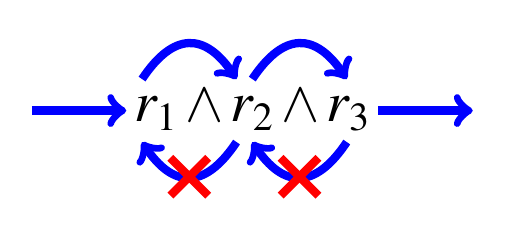
\begin{tikzpicture}[scale=0.8]
          \node[text width=3cm] at (0,0) {\huge $r_1 \wedge r_2 \wedge r_3$};
          \draw [->, line width=3, blue] (-3.5,0) -- (-2,0);
          \draw [->, line width=3, blue] (2,0) -- (3.5,0); 
          \draw [->, line width=3, blue] (-1.75,0.5) .. controls (-1.25,1.25) and (-0.75,1.25) .. (-0.25,0.5);
          \draw [->, line width=3, blue] (-0.25,-0.5) .. controls (-0.75,-1.25) and (-1.25,-1.25) .. (-1.75,-0.5);
          \draw [line width=3, red] (-1.3,-0.75) -- (-0.7,-1.35); 
          \draw [line width=3, red] (-1.3,-1.35) -- (-0.7,-0.75);
          \draw [->, line width=3, blue] (0,0.5) .. controls (0.5,1.25) and (1,1.25) .. (1.5,0.5);
          \draw [->, line width=3, blue] (1.5,-0.5) .. controls (1,-1.25) and (0.5,-1.25) .. (0,-0.5);
          \draw [line width=3, red] (0.45,-0.75) -- (1.05,-1.35); 
          \draw [line width=3, red] (0.45,-1.35) -- (1.05,-0.75);
        \end{tikzpicture}
\end{center}

 \vskip5mm
 
 With optimistic order:
 
 \begin{itemize}
 \item search for answers terminates
 \item search for answers usually is \underline{much} faster
 \end{itemize}

\end{frame}

\begin{frame}[fragile]{Conjucntion non-comutativity}

 \begin{itemize}
 \item It can be not obvious, which order is optimistic
 
  \vskip5mm
  
 \item Optimistic orders can be different for different directions of evaluation
 
  \vskip5mm
  
 \item Optimistic orders can be different on different steps of evaluation
 \end{itemize}

%\begin{center}
\begin{tabular}{ccl}
& & \begin{lstlisting}[escapeinside={(@}{@)},mathescape=true,language=ocaml]
sort$^o$ xs r = ...

perm$^o$ xs ys =
  (fresh (ss) (
     (sort$^o$ xs ss) &&&
     (sort$^o$ ys ss)
  ))
 \end{lstlisting}
\end{tabular}
%\end{center}

\end{frame}

\begin{frame}{Key idea}

Reorder conjuncts
 \begin{itemize}
 \item dynamically
  
 \item conservatively
 
 \item using some divergence test as a signal that order is not optimal
 \end{itemize}
 
 \vskip1cm
 
 \begin{namedthm}{Divergence test}
If relation is called recursively with more general arguments than previous one (i. e. there is a substitution that converts new arguments into old ones) then search for answers will not terminate.
\end{namedthm}

\end{frame}

\begin{frame}[fragile]{Conjunct Reordering Demonstration}
  \begin{tabular}{p{5cm}p{5cm}}
    \begin{lstlisting}[escapeinside={(@}{@)},mathescape=true,language=ocaml]
append$^o$ a b ab =		
  (a === [ ] &&& ab === $\;$b) |||
  fresh (h t tb) 
    (a === h :: t) &&&
    (append$^o$ t b tb) &&&
    (ab === h :: tb)  
  
revers$^o$ a r =	
  (a === [ ] &&& r === [ ]) |||
  fresh (h t rt) 
    (a === h :: t) &&&
    (append$^o$ rt [h] r) &&&
    (revers$^o$ t rt)
\end{lstlisting}
&
\begin{center}
   \Tree [.{\lstinline|revers$^o\; [1,\,2,\,3]\; r$|} ]
\end{center}
\end{tabular}
\end{frame}

\begin{frame}[fragile]{Conjunct Reordering Demonstration}
  \begin{tabular}{p{5cm}p{5cm}}
    \begin{lstlisting}[escapeinside={(@}{@)},mathescape=true,language=ocaml]
append$^o$ a b ab =		
  (a === [ ] &&& ab === $\;$b) |||
  fresh (h t tb) 
    (a === h :: t) &&&
    (append$^o$ t b tb) &&&
    (ab === h :: tb)  
  
revers$^o$ a r =	
  (a === [ ] &&& r === [ ]) |||
  fresh (h t rt) 
    (a === h :: t) &&&
    (append$^o$ rt [h] r) &&&
    (revers$^o$ t rt)
\end{lstlisting}
&
\begin{center}
   \Tree [.{\lstinline|revers$^o\; [1,\,2,\,3]\; r$|}  [.{$[1,\,2,\,3]\not\equiv [\;]$} ] [.{$\ldots$} ] ]
\end{center}
\end{tabular}
\end{frame}

\begin{frame}[fragile]{Conjunct Reordering Demonstration}
  \begin{tabular}{p{5cm}p{5cm}}
    \begin{lstlisting}[escapeinside={(@}{@)},mathescape=true,language=ocaml]
append$^o$ a b ab =		
  (a === [ ] &&& ab === $\;$b) |||
  fresh (h t tb) 
    (a === h :: t) &&&
    (append$^o$ t b tb) &&&
    (ab === h :: tb)  
  
revers$^o$ a r =	
  (a === [ ] &&& r === [ ]) |||
  fresh (h t rt) 
    (a === h :: t) &&&
    (append$^o$ rt [h] r) &&&
    (revers$^o$ t rt)
\end{lstlisting}
&
\begin{center}
   \Tree [.{\lstinline|revers$^o\; [1,\,2,\,3]\; r$|}  [.{$[1,\,2,\,3]\not\equiv [\;]$} ] [.{$[1,\,2,\,3]\equiv h_0:t_0$} ] ]
\end{center}
\end{tabular}
\end{frame}

\begin{frame}[fragile]{Conjunct Reordering Demonstration}
  \begin{tabular}{p{5cm}p{5cm}}
    \begin{lstlisting}[escapeinside={(@}{@)},mathescape=true,language=ocaml]
append$^o$ a b ab =		
  (a === [ ] &&& ab === $\;$b) |||
  fresh (h t tb) 
    (a === h :: t) &&&
    (append$^o$ t b tb) &&&
    (ab === h :: tb)  
  
revers$^o$ a r =	
  (a === [ ] &&& r === [ ]) |||
  fresh (h t rt) 
    (a === h :: t) &&&
    (append$^o$ rt [h] r) &&&
    (revers$^o$ t rt)
\end{lstlisting}
&
\begin{center}
  \Tree [.{\lstinline|revers$^o\; [1,\,2,\,3]\; r$|}
    [.{$[1,\,2,\,3]\not\equiv [\;]$} ]
    [.{$[1,\,2,\,3]\equiv h_0:t_0$}
      [.{\lstinline|append$^o\;rt_0\;[1]\;r$|} ]
    ]
  ]
\end{center}
\end{tabular}
\end{frame}

\begin{frame}[fragile]{Conjunct Reordering Demonstration}
  \begin{tabular}{p{5cm}p{5cm}}
    \begin{lstlisting}[escapeinside={(@}{@)},mathescape=true,language=ocaml]
append$^o$ a b ab =		
  (a === [ ] &&& ab === $\;$b) |||
  fresh (h t tb) 
    (a === h :: t) &&&
    (append$^o$ t b tb) &&&
    (ab === h :: tb)  
  
revers$^o$ a r =	
  (a === [ ] &&& r === [ ]) |||
  fresh (h t rt) 
    (a === h :: t) &&&
    (append$^o$ rt [h] r) &&&
    (revers$^o$ t rt)
\end{lstlisting}
&
\begin{center}
  \Tree [.{\lstinline|revers$^o\; [1,\,2,\,3]\; r$|}
    [.{$[1,\,2,\,3]\not\equiv [\;]$} ]
    [.{$[1,\,2,\,3]\equiv h_0:t_0$}
      [.{\lstinline|append$^o\;rt_0\;[1]\;r$|}
        [.{$\dots$} ]
        [.{$rt_0\equiv h_1:t_1$} [.{\lstinline|append$^o\;t_1\;[1]\;tb_0$|} ] ]
      ]
    ]
  ]
\end{center}
\end{tabular}
\end{frame}


\begin{frame}[fragile]{Conjuncts reordering}

\begin{onlyenv}<1-3>
\begin{lstlisting}[escapeinside={(@}{@)},mathescape=true,language=ocaml]
append$^o$ a b ab =			$\only<2-3>{{\bf a = ?, \;b = ?, \;ab = [1, 2]}}$
  (a === [ ] &&& ab === $\;$b) |||
  (fresh (h t tb) (
     (a === h :: t) &&&
     (append$^o$ t b tb) &&&		$\only<3>{{\bf t = ?, \;b = ?, \;tb = ?}}$
     (ab === h :: tb)  
  ))
 \end{lstlisting}
 \end{onlyenv}
 \begin{onlyenv}<4-5>
\begin{lstlisting}[escapeinside={(@}{@)},mathescape=true,language=ocaml]
append$^o$ a b ab =			$\only<4-5>{{\bf a = ?, \;b = ?, \;ab = [1, 2]}}$
  (a === [ ] &&& ab === $\;$b) |||
  (fresh (h t tb) (
     (a === h :: t) &&&
     (@\color{blue}(ab $\equiv$ h :: tb) $\wedge$@)
     (@\color{blue}(append$^o$ t b tb)@)		   $\only<5>{{\bf t = ?, \;b = ?, \;tb = [2]}}$
  ))
 \end{lstlisting}
 \end{onlyenv}

\end{frame}

\begin{frame}[fragile]{Conjuncts reordering 2}

\begin{onlyenv}<1-5>
\begin{lstlisting}[escapeinside={(@}{@)},mathescape=true,language=ocaml]
append$^o$ a b ab =			$\only<4-5>{{\bf a = ?, \;b = [1], \;ab = ?}}$
  (a === [ ] &&& ab === $\;$b) |||
  (fresh (h t tb) (
     (a === h :: t) &&&
     (append$^o$ t b tb) &&&		$\only<5>{{\bf t = ?, \;b = [1], \;tb = ?}}$
     (ab === h :: tb)  
  ))

revers$^o$ a r =			$\only<2-5>{{\bf a = [1, 2, 3], \;r = ?}}$
  (a === [ ] &&& r === [ ]) |||
  (fresh (h t rt) (
     (a === h :: t) &&&
     (append$^o$ rt [h] r) &&&	$\only<3-4>{{\bf rt = ?, \;h = 1, \;r = ?}}$
     (revers$^o$ t rt)
  ))
 \end{lstlisting}
 \end{onlyenv}
 \begin{onlyenv}<6-7>
\begin{lstlisting}[escapeinside={(@}{@)},mathescape=true,language=ocaml]
append$^o$ a b ab =			$\only<6-7>{{\bf a = ?, \;b = [1], \;ab = ?}}$
  (a === [ ] &&& ab === $\;$b) |||
  (fresh (h t tb) (
     (a === h :: t) &&&
     (@\color{blue}(ab $\equiv$ h :: tb) $\wedge$@)
     (@\color{blue}(append$^o$ t b tb)@)		   $\only<7>{{\bf t = ?, \;b = [1], \;tb = ?}}$
  ))

revers$^o$ a r =			$\only<6-7>{{\bf a = [1, 2, 3], \;r = ?}}$
  (a === [ ] &&& r === [ ]) |||
  (fresh (h t rt) (
     (a === h :: t) &&&
     (append$^o$ rt [h] r) &&&
     (revers$^o$ t rt)
  ))
 \end{lstlisting}
 \end{onlyenv}
 \begin{onlyenv}<8-9>
\begin{lstlisting}[escapeinside={(@}{@)},mathescape=true,language=ocaml]
append$^o$ a b ab =
  (a === [ ] &&& ab === $\;$b) |||
  (fresh (h t tb) (
     (a === h :: t) &&&
     (append$^o$ t b tb) &&&
     (ab === h :: tb)  
  ))

revers$^o$ a r =			$\only<8-9>{{\bf a = [1, 2, 3], \;r = ?}}$
  (a === [ ] &&& r === [ ]) |||
  (fresh (h t rt) (
     (a === h :: t) &&&
     (@\color{blue}(revers$^o$ t rt) $\wedge$@)		    $\only<9>{{\bf t = [2, 3], \;r = ?}}$
     (@\color{blue}(append$^o$ rt [h] r)@)
  ))
 \end{lstlisting}
 \end{onlyenv}

\end{frame}

\begin{frame}{Formal development}

Operational semantics (for terminating programs only!):
 \begin{itemize}
 \item standart search
 \item search with extension
 \end{itemize}
 
 \vskip1cm
 
 Proofs:
 \begin{itemize}
 \item divergence test
 \item extension preserves termination
 \end{itemize}
 
\end{frame}

\begin{frame}{Evaluation}

Implemented for OCanren (typed MiniKanren for OCaml)

 \vskip8mm

Test detects divergence in all natural relations (only artificial counterexamples)

 \vskip8mm

Fixed relations:
 \begin{itemize}
 \item list relations (append, reverse, map)
 \item list sorting
 \item binary arithmetic (addition, multiplication, division, comparisons)
 \item binary tree size
 \end{itemize}
 
\end{frame}

\begin{frame}{Contributions}

\begin{itemize}
 \item Divergence test and conjuncts reordering algorithm based on it
 \vskip1cm
 \item Operational semantics and proofs of divergence test and termination preservation
 \vskip1cm
 \item Evaluation
\end{itemize}
 
\end{frame}


\end{document}
